% Chapter 4
\chapter{نتایج}

در فصل قبل، جزئیات مدل پیشنهادی برای پیش‌بینی تداخلات دارویی ارائه شد. این مدل با ترکیب اطلاعات ساختاری، شباهت دارویی و داده‌های متنی، یک رویکرد چندوجهی برای شناسایی تداخلات دارویی ارائه می‌دهد. در این فصل، به منظور ارزیابی جامع قابلیت‌های مدل پیشنهادی، عملکرد آن در شرایط مختلف مورد بررسی قرار می‌گیرد. برای این منظور، سه سناریوی متفاوت طراحی شده است که هر کدام جنبه‌های خاصی از توانایی‌های مدل را می‌سنجند. سپس نتایج حاصل از این ارزیابی‌ها با روش‌های موجود مقایسه شده و مورد تحلیل قرار می‌گیرند.

این فصل در شش بخش اصلی سازماندهی شده است: در بخش اول، جزئیات سناریوهای ارزیابی مدل تشریح می‌شود. در بخش دوم، نتایج مدل پیشنهادی با روش‌های موجود مقایسه می‌گردد. در بخش سوم، با انجام مطالعه تقطیعی، تأثیر هر یک از اجزای مدل در عملکرد نهایی مورد بررسی قرار می‌گیرد. بخش چهارم به تفسیر نتایج و تحلیل عمیق‌تر یافته‌ها می‌پردازد. در بخش پنجم، تحلیل رابطه بین شباهت دارویی و تداخلات ارائه می‌شود. در نهایت، در بخش ششم چالش‌های موجود در پیش‌بینی تداخلات دارویی و محدودیت‌های فعلی مورد بحث قرار می‌گیرند.

\section{سناریوهای ارزیابی مدل}

برای ارزیابی جامع مدل پیشنهادی و سنجش قابلیت آن در شرایط مختلف کاربردی، سه سناریوی متفاوت طراحی شده است. این سناریوها که از حالت‌های ساده تا پیچیده را پوشش می‌دهند، با تقسیم‌بندی متفاوت داده‌ها به مجموعه‌های آموزش و آزمون، شرایط واقعی استفاده از مدل را شبیه‌سازی می‌کنند. هر سناریو با هدف سنجش جنبه خاصی از عملکرد مدل، از جمله توانایی تعمیم به داروهای جدید و قابلیت پیش‌بینی در شرایط مختلف طراحی شده است. مجموعه داده مورد استفاده در این پژوهش شامل اطلاعات 936 دارو و بیش از 103,000 تداخل شناسایی شده بین این داروها است که برای ارزیابی مدل در سناریوهای مختلف مورد استفاده قرار گرفته است.


\subsection{سناریوی اول: اعتبارسنجی متقاطع K-Fold}

در سناریوی اول، از روش اعتبارسنجی متقاطع \lr{K-Fold} با مقدار $K=5$ برای تقسیم‌بندی تداخلات دارویی استفاده شده است. همان‌طور که در شکل \ref{fig:senario-1} نشان داده شده است، در این روش کل مجموعه تداخلات دارویی به پنج بخش مساوی تقسیم می‌شود. در هر تکرار، یکی از این بخش‌ها به عنوان مجموعه آزمون و چهار بخش دیگر به عنوان مجموعه آموزش در نظر گرفته می‌شوند. این فرآیند پنج بار تکرار می‌شود، به طوری که هر بخش دقیقاً یک بار نقش مجموعه آزمون را ایفا می‌کند. نکته قابل توجه در این سناریو این است که تقسیم‌بندی بر اساس تداخلات دارویی انجام می‌شود، نه داروها؛ به این معنی که یک دارو می‌تواند هم در مجموعه آموزش و هم در مجموعه آزمون حضور داشته باشد. این موضوع محدودیت قابل توجهی برای ارزیابی مدل ایجاد می‌کند، زیرا مدل در مرحله آموزش می‌تواند تا حدودی با الگوهای تداخلی داروهای موجود در مجموعه آزمون آشنا شده باشد. به همین دلیل، برای ارزیابی واقعی‌تر قابلیت تعمیم مدل به داروهای جدید، نیاز به طراحی سناریوهای پیچیده‌تر احساس می‌شود.

\begin{figure}[t]
	\centering
	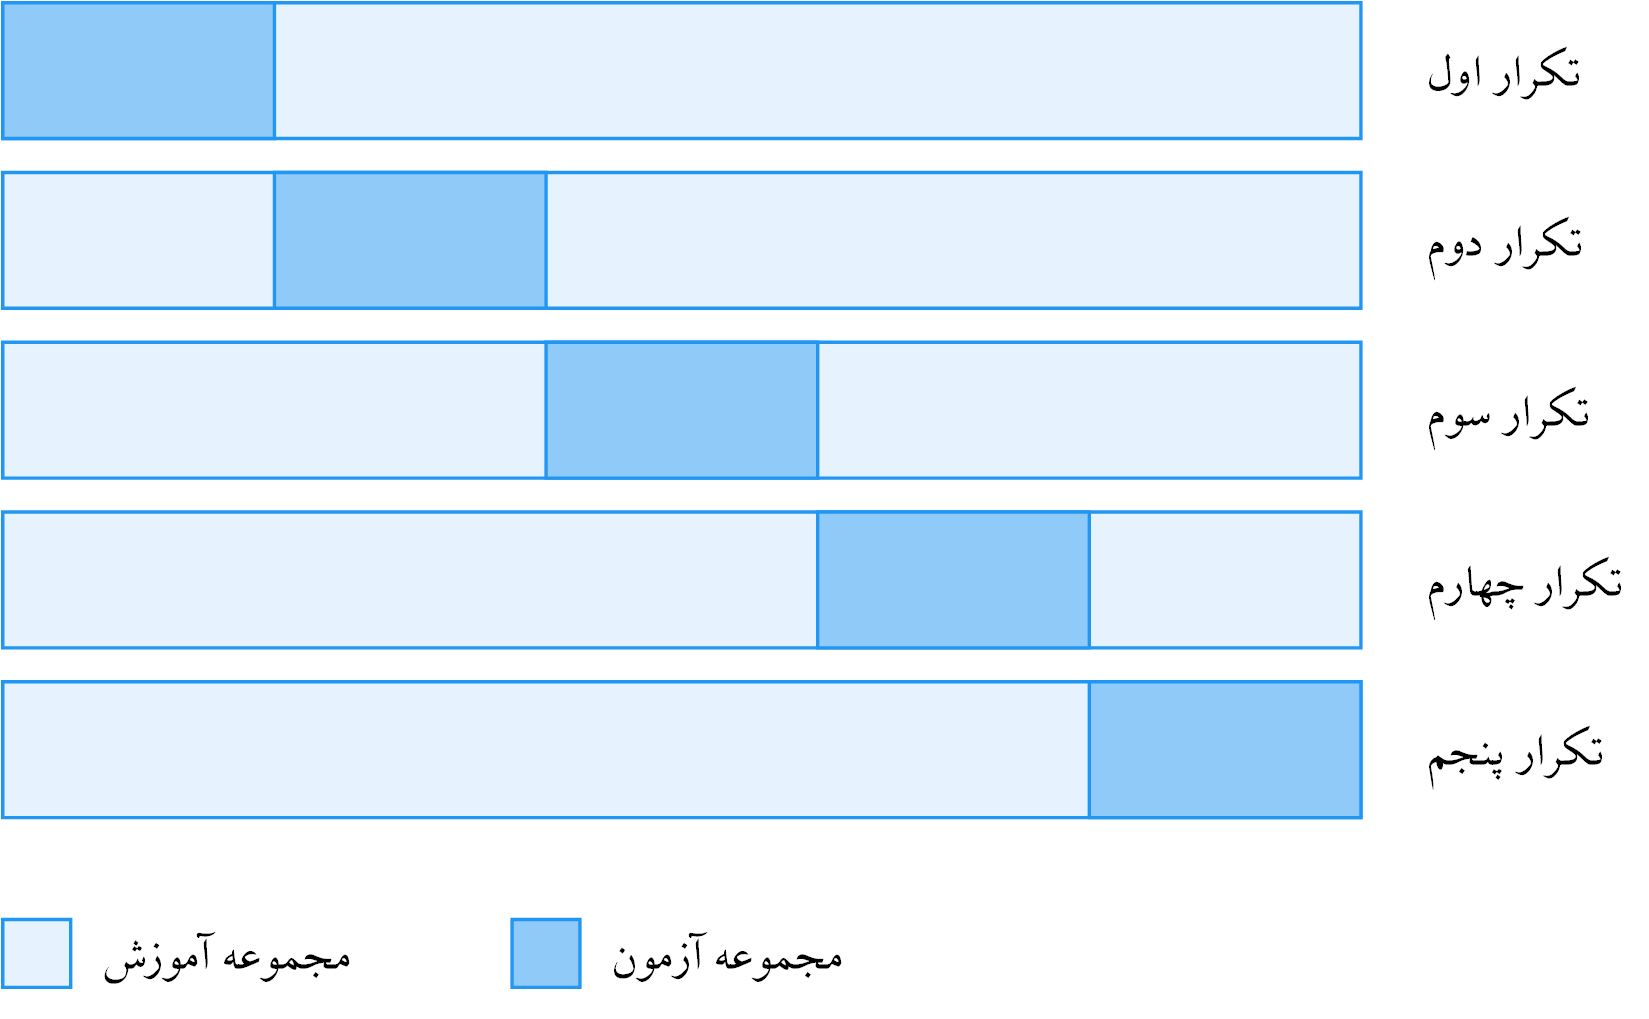
\includegraphics[width=\textwidth]{images/senario-1.png}
	\caption{نحوه تقسیم‌بندی داده‌ها در سناریوی اول با استفاده از اعتبارسنجی متقاطع \lr{5-Fold}}
	\label{fig:senario-1}
\end{figure}

\subsection{سناریوی دوم: تقسیم‌بندی بر اساس داروها با داده‌های جدید در آزمون}

\begin{figure}[t]
	\centering
	\begin{subfigure}[b]{0.42\textwidth} % Adjusted width to fit side by side
		\centering
		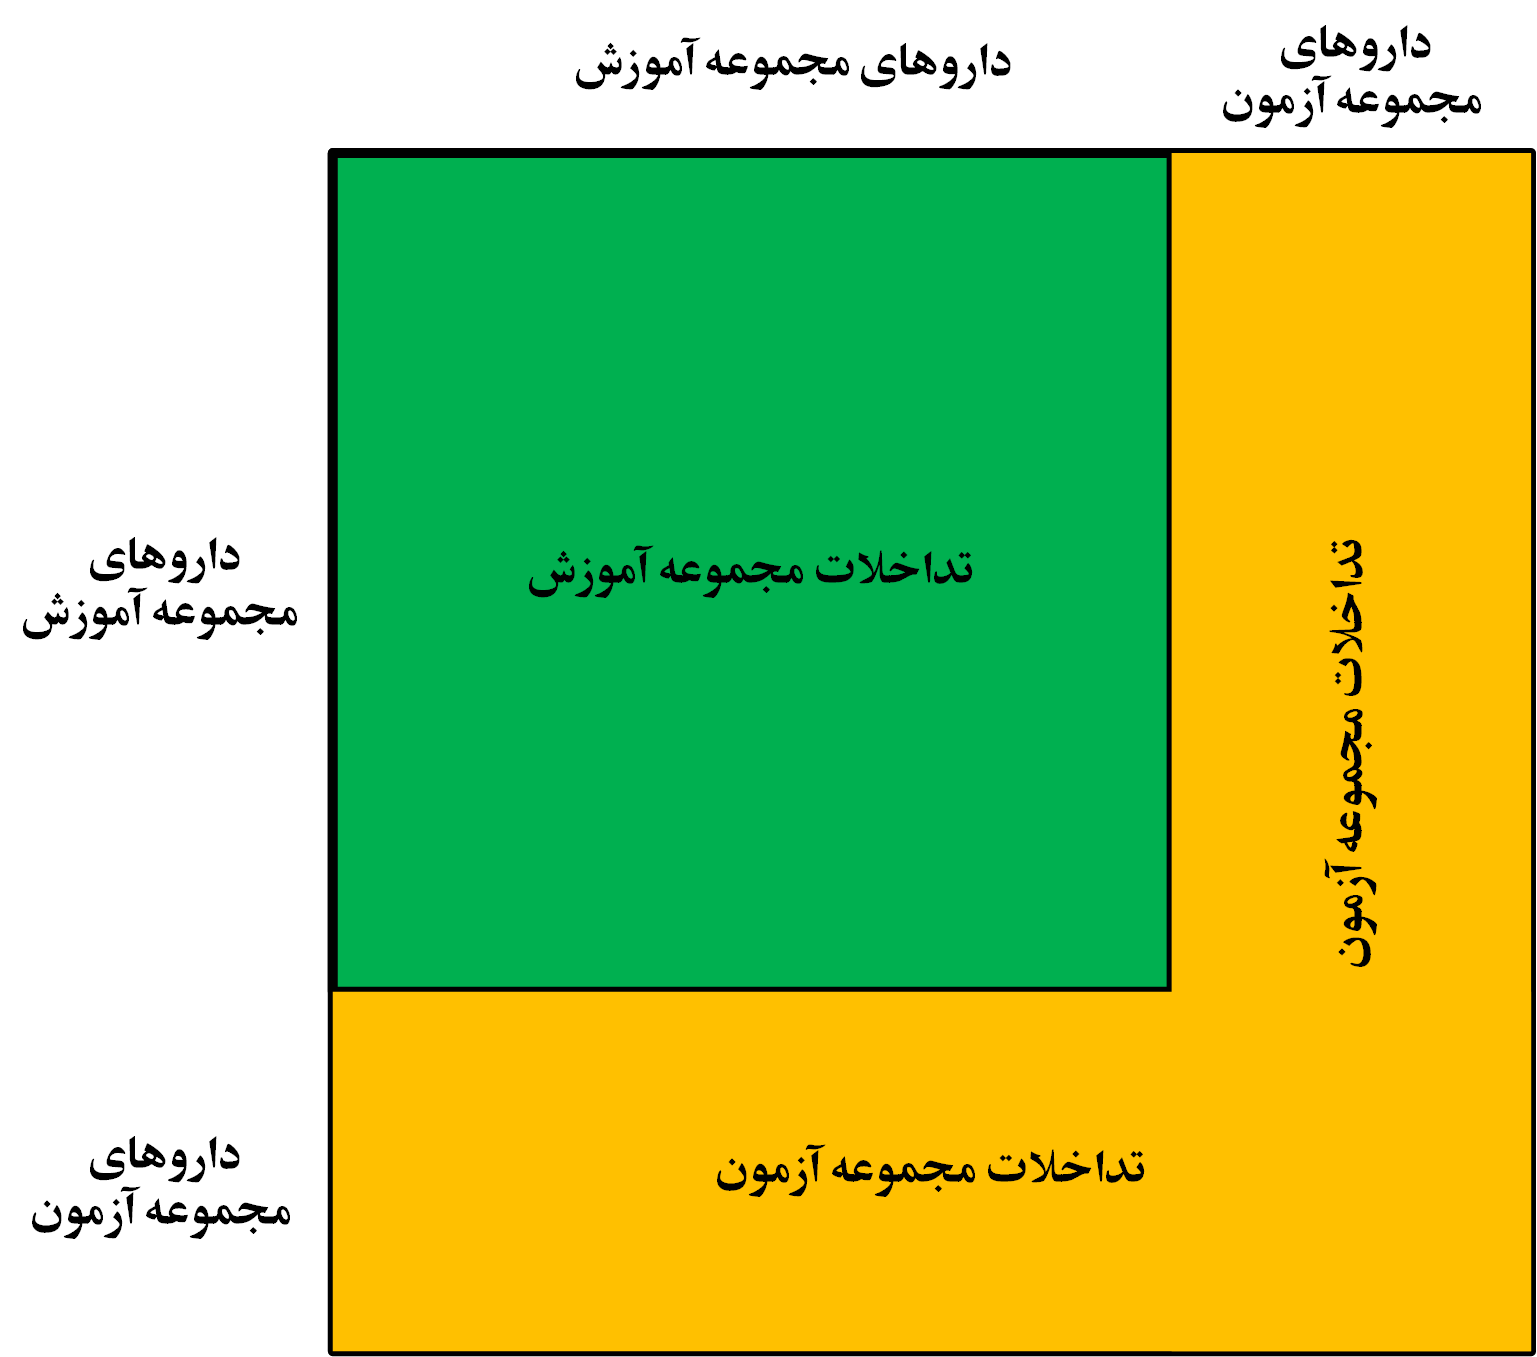
\includegraphics[width=\textwidth]{images/senario-2-matrix.png}
		\caption{نمایش ماتریسی نحوه تقسیم‌بندی داده‌ها}
		\label{fig:senario-2-matrix}
	\end{subfigure}
	\hspace{0.04\textwidth} % Optional spacing between the subfigures
	\begin{subfigure}[b]{0.42\textwidth} % Adjusted width to fit side by side
		\centering
		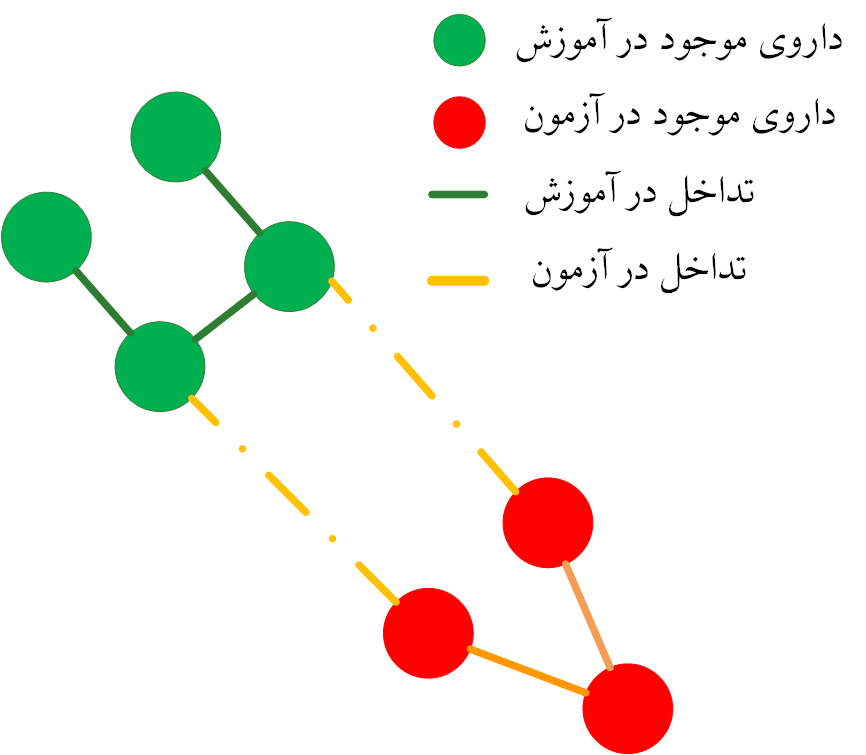
\includegraphics[width=\textwidth]{images/senario-2-graph.png}
		\caption{نمایش گرافی نحوه تقسیم‌بندی داده‌ها}
		\label{fig:senario-2-graph}
	\end{subfigure}
	\caption{نحوه تقسیم‌بندی داده‌ها در سناریوی دوم}
	\label{fig:senario-2}
\end{figure}

سناریوی دوم با هدف غلبه بر محدودیت اصلی سناریوی اول طراحی شده است. همان‌طور که در شکل \ref{fig:senario-2} نشان داده شده است، در این سناریو داروها (نه تداخلات) به دو دسته مجموعه آموزش و آزمون تقسیم می‌شوند. در مجموعه آموزش، تنها تداخلات بین داروهای موجود در مجموعه آموزش در نظر گرفته می‌شوند. در مجموعه آزمون، تمام تداخلات مربوط به داروهای مجموعه آزمون مورد بررسی قرار می‌گیرند، حتی اگر یک طرف تداخل مربوط به داروهای مجموعه آموزش باشد.

برای پیاده‌سازی این سناریو، ابتدا داروها با استفاده از یک تابع سفارشی شبیه به الگوریتم \lr{K-Fold}، با $K=5$، به پنج زیرمجموعه تقسیم می‌شوند. سپس، در هر تکرار، یک زیرمجموعه به عنوان مجموعه آزمون و چهار زیرمجموعه دیگر به عنوان مجموعه آموزش در نظر گرفته می‌شوند. به این ترتیب، مدل در مرحله آزمون با داروهایی مواجه می‌شود که در هنگام آموزش ندیده است. این سناریو، شبیه‌سازی بهتری از شرایط دنیای واقعی ارائه می‌دهد که در آن ممکن است پزشکان با تجویز ترکیبات دارویی جدید مواجه شوند. همچنین برای اطمینان از وجود داده‌های کافی در مجموعه آزمون، تنها تداخلاتی در نظر گرفته شدند که حداقل 50 نمونه برای آن‌ها موجود بود. این محدودیت منجر به کاهش تعداد انواع تداخلات از 65 به 47 نوع شد، اما اطمینان حاصل شد که برای هر نوع تداخل، داده‌های کافی برای ارزیابی معتبر مدل وجود دارد.

\subsection{سناریوی سوم: تقسیم‌بندی بر اساس داروها با هر دو دارو از مجموعه آزمون}

سناریوی سوم، با هدف ارزیابی عملکرد مدل در سخت‌ترین شرایط ممکن طراحی شده است. همان‌طور که در شکل \ref{fig:senario-3} نشان داده شده است، در این سناریو مانند سناریوی دوم، داروها به دو دسته مجموعه آموزش و آزمون تقسیم می‌شوند. با این تفاوت که در مجموعه آزمون، تنها تداخلاتی مورد ارزیابی قرار می‌گیرند که هر دو داروی مرتبط با آنها در مجموعه آزمون قرار دارند. این شرایط، بالاترین سطح چالش را برای مدل ایجاد می‌کند زیرا هیچ یک از داروهای موجود در تداخلات مورد آزمون، در مرحله آموزش توسط مدل دیده نشده‌اند.

در این سناریو، به دلیل محدودیت شدیدتر در انتخاب تداخلات دارویی، نیاز به داده‌های بیشتر برای هر نوع تداخل وجود داشت. بنابراین، تنها تداخلاتی در نظر گرفته شدند که حداقل 400 نمونه برای آن‌ها موجود بود. این محدودیت تعداد انواع تداخلات را از 65 به 18 نوع کاهش داد، اما این کاهش برای اطمینان از وجود داده‌های کافی برای ارزیابی معتبر در این سناریوی چالش‌برانگیز ضروری بود. سناریوهای دوم و سوم، مشابه با رویکردهای استفاده شده در \cite{ref_deng2020} هستند، که نشان‌دهنده اهمیت ارزیابی عملکرد مدل در مواجهه با داروهای کاملاً جدید است.

ارزیابی عملکرد مدل پیشنهادی در این سه سناریو، امکان بررسی جامع قابلیت‌های مدل در شرایط مختلف را فراهم می‌کند. در حالی که سناریوی اول، یک رویکرد استاندارد برای ارزیابی کلی مدل ارائه می‌دهد، سناریوهای دوم و سوم با شبیه‌سازی شرایط واقعی‌تر، توانایی مدل را در مواجهه با داروهای جدید می‌سنجند. این موضوع به ویژه از آن جهت اهمیت دارد که در محیط‌های بالینی واقعی، پزشکان اغلب با ترکیبات دارویی جدید مواجه می‌شوند.

هر یک از این سناریوها محدودیت‌های خاص خود را نیز دارند. در سناریوهای دوم و سوم، با افزایش سطح چالش برای مدل و اعمال محدودیت‌های بیشتر در انتخاب داده‌ها، تعداد نمونه‌های موجود در مجموعه آزمون و تعداد انواع تداخلات قابل بررسی کاهش می‌یابد. با این وجود، نتایج به دست آمده از این سناریوها می‌توانند در توسعه بیشتر مدل و ارزیابی قابلیت کاربرد آن در محیط‌های واقعی نقش مهمی ایفا کنند. تحلیل عمیق‌تر این نتایج و پیامدهای آنها برای کاربردهای عملی مدل در بخش‌های بعدی این فصل ارائه خواهد شد.


\begin{figure}[!t]
	\centering
	\begin{subfigure}[b]{0.42\textwidth} % Adjusted width to fit side by side
		\centering
		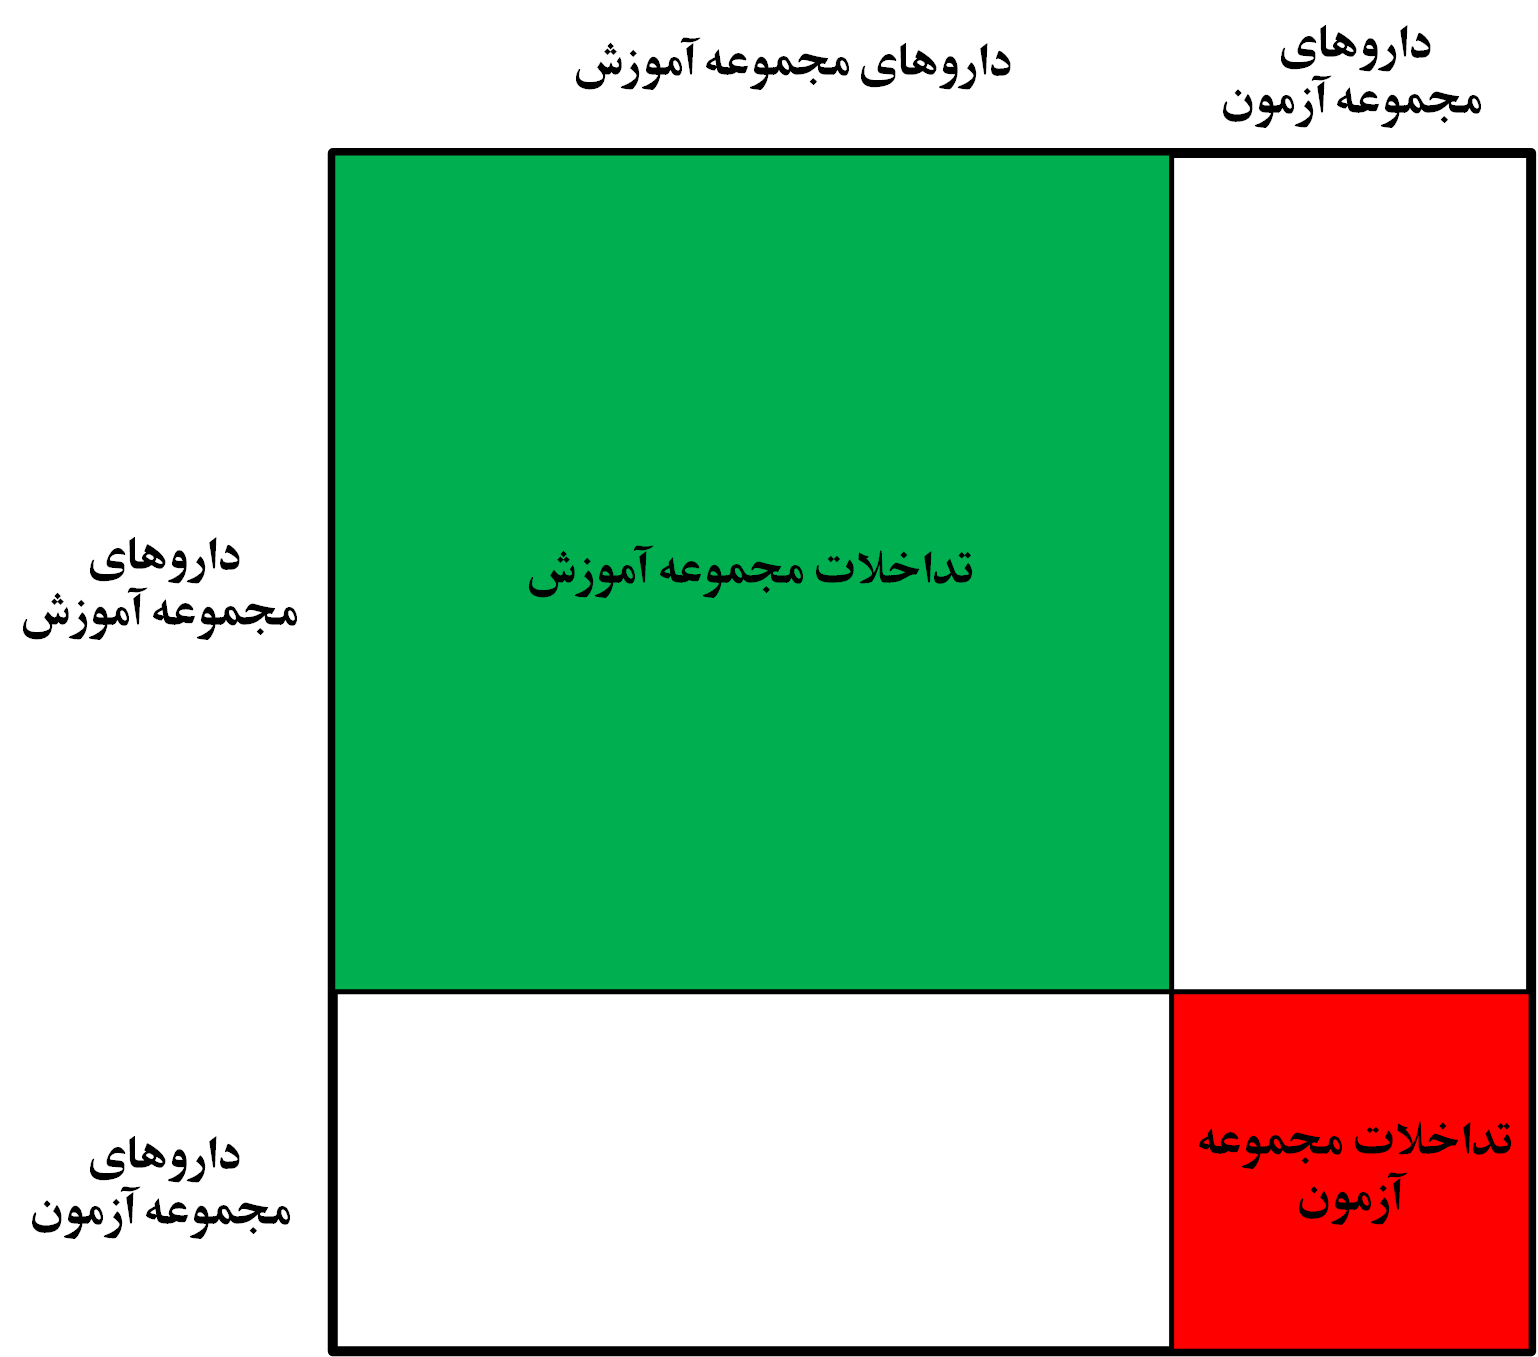
\includegraphics[width=\textwidth]{images/senario-3-matrix.png}
		\caption{نمایش ماتریسی نحوه تقسیم‌بندی داده‌ها}
		\label{fig:senario-3-matrix}
	\end{subfigure}
	\hspace{0.04\textwidth} % Optional spacing between the subfigures
	\begin{subfigure}[b]{0.42\textwidth} % Adjusted width to fit side by side
		\centering
		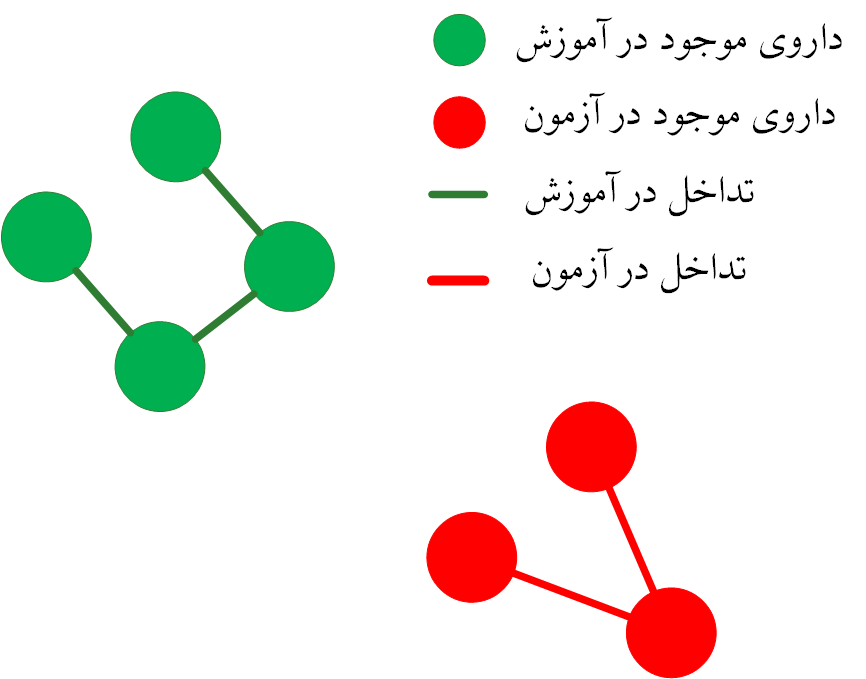
\includegraphics[width=\textwidth]{images/senario-3-graph.png}
		\caption{نمایش گرافی نحوه تقسیم‌بندی داده‌ها}
		\label{fig:senario-3-graph}
	\end{subfigure}
	\caption{نحوه تقسیم‌بندی داده‌ها در سناریوی سوم}
	\label{fig:senario-3}
\end{figure}


\section{مقایسه با روش‌های موجود}

برای ارزیابی جامع عملکرد مدل پیشنهادی، نتایج آن با دو گروه مختلف از مدل‌ها مقایسه شده است. گروه اول شامل مدل‌های پیشرفته و تخصصی در حوزه تداخلات دارویی است که از این میان می‌توان به \lr{DeepDDI} \cite{ref_ryu2018} و \lr{DDIMDL} \cite{ref_deng2020} اشاره کرد. \lr{DeepDDI} یک مدل یادگیری عمیق است که از شبکه‌های عصبی برای استخراج ویژگی‌های ساختاری داروها استفاده می‌کند، در حالی که \lr{DDIMDL} با بهره‌گیری از رویکرد یادگیری چندوظیفه‌ای، عملکرد پیش‌بینی تداخلات دارویی را بهبود می‌بخشد. این دو مدل از کارآمدترین روش‌های موجود در این حوزه محسوب می‌شوند و مقایسه با آنها می‌تواند معیار مناسبی برای ارزیابی کارایی مدل پیشنهادی باشد.

گروه دوم شامل الگوریتم‌های پایه یادگیری ماشین مانند رگرسیون لجستیک\LTRfootnote{Logistic Regression}، جنگل تصادفی\LTRfootnote{Random Forest} و نزدیک‌ترین همسایه\LTRfootnote{K-Nearest Neighbors} است. مقایسه با این الگوریتم‌های پایه که در بسیاری از مسائل طبقه‌بندی عملکرد قابل قبولی از خود نشان داده‌اند، می‌تواند میزان بهبود عملکرد نسبت به روش‌های متداول را به خوبی نمایان سازد و اهمیت استفاده از روش‌های پیشرفته‌تر را در این حوزه تأیید کند.

نتایج مقایسه‌ها برای هر سه سناریوی تقسیم‌بندی داده‌ها در ادامه به تفصیل مورد بررسی قرار گرفته‌اند. برای ارزیابی جامع عملکرد مدل‌ها، از معیار دقت به عنوان شاخص کلی عملکرد و معیار \lr{F1-Score} برای بررسی دقیق‌تر استفاده شده است. برای درک بهتر عملکرد مدل در هر نوع تداخل، معیار \lr{F1-Score} به صورت \lr{Micro}، \lr{Macro} و \lr{Weighted} برای هر یک از انواع تداخلات به طور جداگانه محاسبه شده است. این معیار با ترکیب نتایج مختلف، تصویر جامع‌تری از عملکرد مدل ارائه می‌دهد و به خصوص در شرایط عدم توازن داده‌ها، ارزیابی دقیق‌تری را ممکن می‌سازد. همچنین با توجه به عدم تعادل قابل توجه در تعداد نمونه‌های هر نوع تداخل، از نمودارهای قطبی\LTRfootnote{Polar} برای نمایش مقدار \lr{F1-Score} مدل‌های مختلف به ازای هر یک از انواع تداخلات استفاده شده است. این نمودارها امکان مقایسه دقیق عملکرد مدل‌ها را در تمامی انواع تداخلات مورد بررسی در هر سناریو فراهم می‌کنند و نشان می‌دهند که مدل پیشنهادی در کدام انواع تداخلات عملکرد بهتری نسبت به سایر مدل‌ها داشته است. جزئیات کامل این معیارها و نحوه محاسبه آن‌ها در پیوست دوم ارائه شده است.

\subsection{نتایج در سناریوی اول}

در سناریوی اول که با استفاده از اعتبارسنجی متقاطع \lr{5-Fold} انجام شد، مدل پیشنهادی عملکرد قابل توجهی را نشان داد. نتایج ارائه شده در جدول \ref{table:scenario2_results} که مقایسه مدل پیشنهادی با سایر مدل‌ها را بر اساس معیارهای دقت و \lr{F1-Score} نشان می‌دهد، حاکی از برتری مدل پیشنهادی در تمامی این معیارها است.

برای بررسی دقیق‌تر عملکرد مدل‌ها در انواع مختلف تداخلات، شکل \ref{fig:s2_f1_score} نتایج معیار \lr{F1-Score} را به صورت نمودار قطبی نمایش می‌دهد. بررسی این نمودار آشکار می‌سازد که مدل پیشنهادی نه تنها در کل عملکرد بهتری داشته، بلکه در اکثر انواع تداخلات، به‌ویژه در مواردی که تعداد نمونه‌های کمتری دارند، نیز توانسته است نسبت به بهترین مدل رقیب (\lr{DDIMDL}) عملکرد بهتری از خود نشان دهد.

\begin{table}[!t]
	\caption{مقایسه نتایج مدل پیشنهادی با سایر مدل‌ها در سناریوی اول}
	\label{table:scenario2_results}
	\centering % برای وسط‌چین کردن جدول
	\renewcommand{\arraystretch}{2.5} 
	\resizebox{0.5\textwidth}{!}{ % Scale table to text width
		\begin{LTR}
			\begin{tabular}{|l|c|ccc|} \hline
				\textbf{Model} & \textbf{Acc} & \multicolumn{3}{c|}{\lr{F1-Score}}\\
				\cline{3-5}
				&  & Mi & Ma & W \\
				\hline
				\lr{DDIMDL} & \lr{94.5} & \lr{94.5} & \lr{92.5} & \lr{94.5} \\ \hline
				\lr{DeepDDI} & \lr{92.5} & \lr{92.5} & \lr{88.8} & \lr{92.5} \\ \hline
				\lr{KNN} & \lr{75.1} & \lr{75.1} & \lr{69.7} & \lr{75.0} \\ \hline
				\lr{LR} & \lr{89.8} & \lr{89.8} & \lr{88.6} & \lr{89.7} \\ \hline
				\lr{RF} & \lr{91.2} & \lr{91.2} & \lr{85.2} & \lr{91.0} \\ \hline
				\lr{Our Model} & \textbf{\lr{96.5}} & \textbf{\lr{96.5}} & \textbf{\lr{94.5}} & \textbf{\lr{96.5}} \\ \hline
			\end{tabular}
		\end{LTR}
	}
\end{table}


\begin{figure}[t]
	\centering
	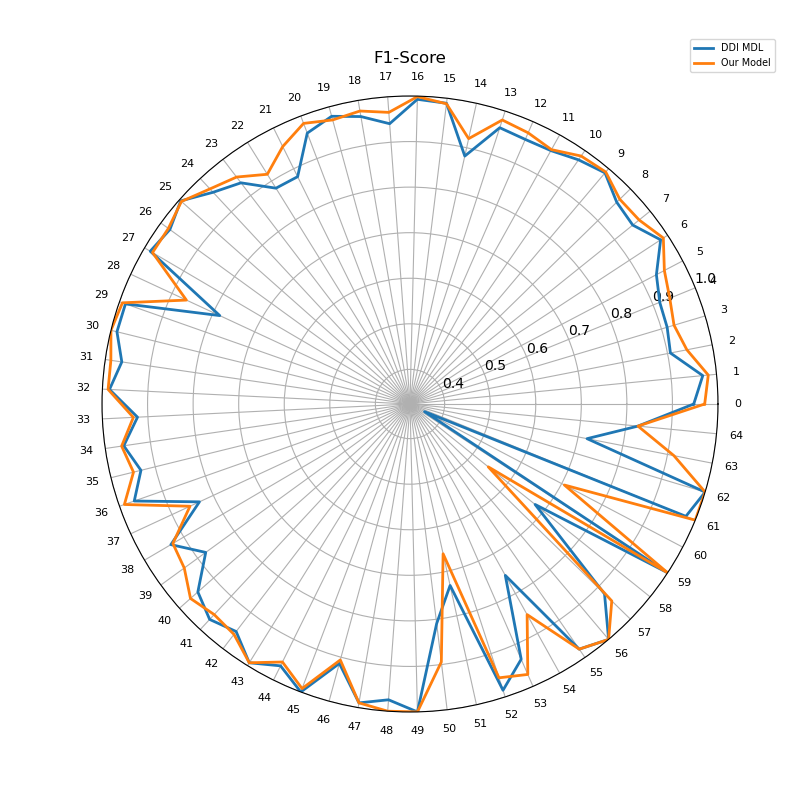
\includegraphics[width=\textwidth]{images/s2-f1-score.png}
	\caption{ امتیاز F1 در انواع مختلف برای سناریو اول }
	\label{fig:s2_f1_score}
\end{figure}

\subsection{نتایج در سناریوی دوم}

با توجه به سناریوهای ارزیابی که در بخش‌های قبل‌ معرفی شدند، سناریوی دوم با هدف ارزیابی توانایی مدل در پیش‌بینی تداخلات برای داروهای جدید طراحی شده است. نتایج ارائه شده در جدول \ref{table:scenario3_results} که مقایسه مدل پیشنهادی با سایر مدل‌ها را بر اساس معیارهای دقت و \lr{F1-Score} نشان می‌دهد، حاکی از برتری مدل پیشنهادی در تمامی این معیارها است.

\begin{table}[t]
	\caption{مقایسه نتایج مدل پیشنهادی با سایر مدل‌ها در سناریوی دوم}
	\label{table:scenario3_results}
	\centering % برای وسط‌چین کردن جدول
	\renewcommand{\arraystretch}{2.5} 
	\resizebox{0.5\textwidth}{!}{ % Scale table to text width
		\begin{LTR} % Force LTR direction for the table
			\begin{tabular}{|l|c|ccc|} \hline
				\textbf{Model} & \textbf{Acc} & \multicolumn{3}{c|}{\lr{F1-Score}}\\
				\cline{3-5}
				&  & Mi & Ma & W \\
				\hline
				\lr{DDIMDL} & \lr{68.6} & \lr{68.6} & \lr{66.5} & \lr{67.6} \\ \hline
				\lr{DeepDDI} & \lr{26.8} & \lr{26.8} & \lr{0.9} & \lr{11.4} \\ \hline
				\lr{KNN} & \lr{63.0} & \lr{63.0} & \lr{56.9} & \lr{62.1} \\ \hline
				\lr{LR} & \lr{64.7} & \lr{64.7} & \lr{64.7} & \lr{63.8} \\ \hline
				\lr{RF} & \lr{68.9} & \lr{68.9} & \lr{66.3} & \lr{67.8} \\ \hline
				\lr{Our Model} & \textbf{\lr{69.8}} & \textbf{\lr{69.8}} & \textbf{\lr{66.6}} & \textbf{\lr{68.9}} \\ \hline
			\end{tabular}
		\end{LTR} 
	}
\end{table}

برای تحلیل دقیق‌تر عملکرد مدل‌ها، شکل \ref{fig:s3_f1_score} توزیع معیار \lr{F1-Score} را در قالب نمودار قطبی برای انواع مختلف تداخلات نمایش می‌دهد. این نمودار نشان می‌دهد که مدل پیشنهادی حتی در این سناریوی چالش‌برانگیز نیز توانسته است در اکثر انواع تداخلات، نسبت به بهترین مدل رقیب (\lr{DDIMDL}) عملکرد بهتری را به ثبت برساند، که این امر نشان‌دهنده قابلیت تعمیم‌پذیری مناسب مدل پیشنهادی است.

\begin{figure}[t]
	\centering
	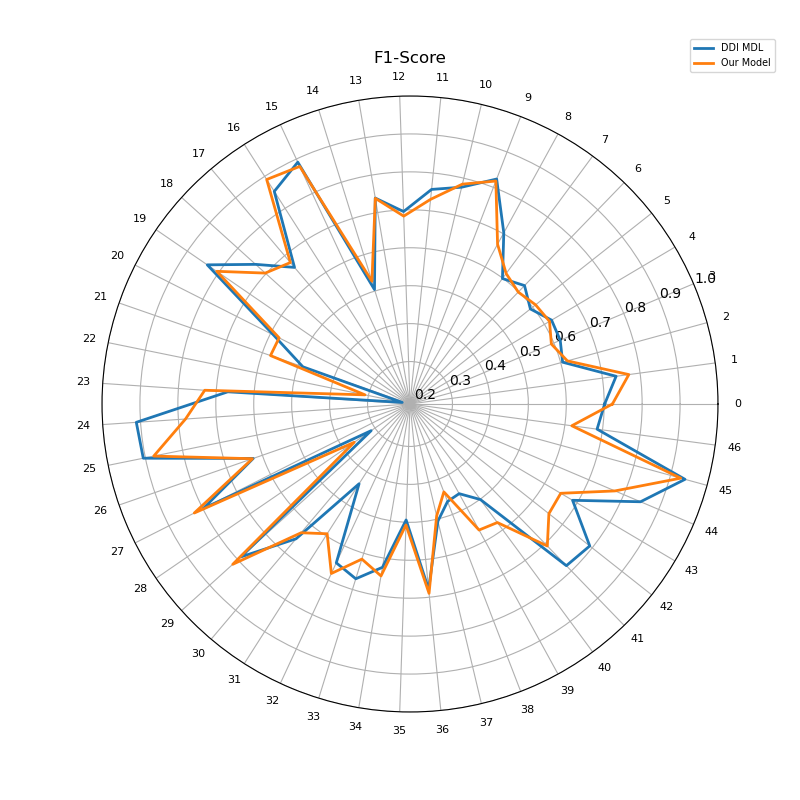
\includegraphics[width=\textwidth]{images/s3-f1-score.png}
	\caption{ امتیاز F1 در انواع مختلف برای سناریو دوم }
	\label{fig:s3_f1_score}
\end{figure}

\subsection{نتایج در سناریوی سوم}

سناریوی سوم به عنوان چالش‌برانگیزترین حالت ارزیابی مدل، با هدف بررسی عملکرد آن در شرایطی طراحی شده است که هر دو داروی درگیر در تداخل‌های مورد آزمایش برای مدل ناشناخته هستند. در این سناریو، با اعمال محدودیت‌های شدیدتر در انتخاب داده‌های آزمون، مجموعه داده محدودتری نسبت به سناریوهای قبلی مورد استفاده قرار گرفت. با وجود این شرایط دشوار، نتایج ارائه شده در جدول \ref{table:scenario4_results} همچنان حاکی از برتری مدل پیشنهادی در معیارهای دقت و \lr{F1-Score} نسبت به سایر روش‌هاست.

\begin{table}[t]
	\caption{مقایسه نتایج مدل پیشنهادی با سایر مدل‌ها در سناریوی سوم}
	\label{table:scenario4_results}
	\centering % برای وسط‌چین کردن جدول
	\renewcommand{\arraystretch}{2.5} 
	\resizebox{0.5\textwidth}{!}{ % Scale table to text width
		\begin{LTR}
			\begin{tabular}{|l|c|ccc|} \hline
				\textbf{Model} & \textbf{Acc} & \multicolumn{3}{c|}{\lr{F1-Score}} \\
				\cline{3-5}
				&  & Mi & Ma & W \\
				\hline
				\lr{DDIMDL} & \lr{50.2} & \lr{50.2} & \textbf{\lr{45.0}} & \lr{47.4} \\ \hline
				\lr{DeepDDI} & \lr{26.7} & \lr{26.7} & \lr{2.3} & \lr{11.4} \\ \hline
				\lr{KNN} & \lr{45.4} & \lr{45.4} & \lr{36.5} & \lr{43.8} \\ \hline
				\lr{LR} & \lr{46.6} & \lr{46.6} & \lr{41.9} & \lr{44.2} \\ \hline
				\lr{RF} & \lr{47.7} & \lr{47.7} & \lr{37.6} & \lr{43.7} \\ \hline
				\lr{Our Model} & \textbf{\lr{50.8}} & \textbf{\lr{50.8}} & \lr{44.3} & \textbf{\lr{48.4}} \\ \hline
			\end{tabular}
		\end{LTR}
	}
\end{table}

برای تحلیل عمیق‌تر عملکرد مدل‌ها در این سناریوی دشوار، شکل \ref{fig:s4_f1_score} توزیع معیار \lr{F1-Score} را در قالب نمودار قطبی برای انواع مختلف تداخلات نمایش می‌دهد. بررسی این نمودار نشان می‌دهد که مدل پیشنهادی، حتی در این شرایط که هر دو دارو برای مدل جدید هستند، توانسته است در اکثر انواع تداخلات عملکرد بهتری نسبت به بهترین مدل رقیب (\lr{DDIMDL}) از خود نشان دهد، که این امر حاکی از توانایی قابل توجه مدل در تعمیم‌پذیری به داروهای کاملاً جدید است.

\begin{figure}[t]
	\centering
	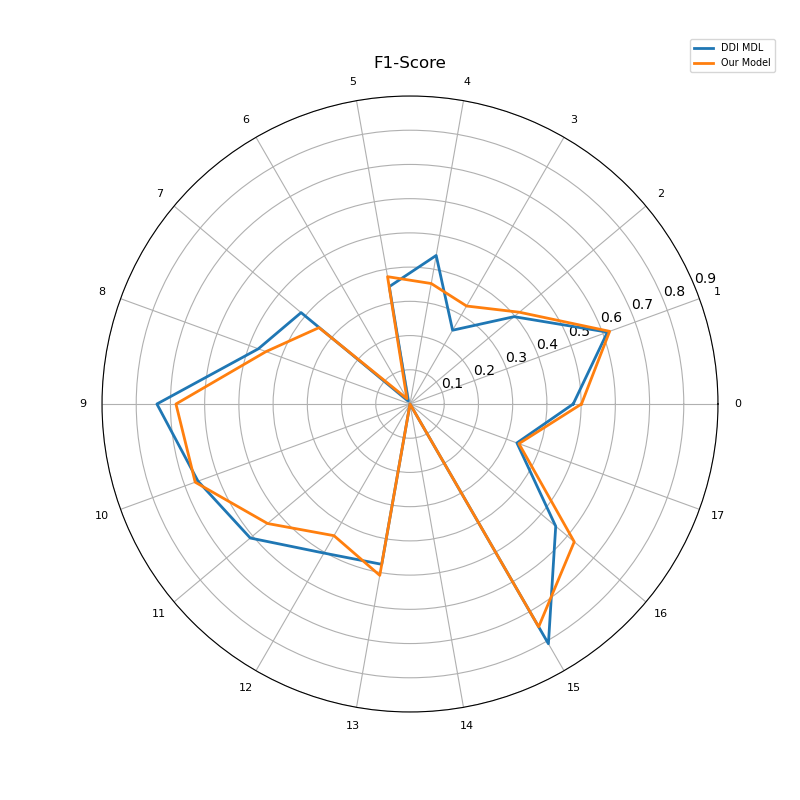
\includegraphics[width=\textwidth]{images/s4-f1-score.png}
	\caption{ امتیاز F1 در انواع مختلف برای سناریو سوم }
	\label{fig:s4_f1_score}
\end{figure}

\subsection{تحلیل مقایسه‌ای نتایج}

نتایج حاصل از سه سناریوی مختلف نشان می‌دهند که مدل پیشنهادی در تمامی شرایط عملکرد بهتری نسبت به سایر مدل‌ها داشته است. این برتری حتی در سناریوهای دوم و سوم که شرایط ارزیابی سخت‌گیرانه‌تری دارند نیز مشهود است. در این میان، مدل‌های پایه مانند جنگل تصادفی و نزدیک‌ترین همسایه عملکرد ضعیف‌تری در مقایسه با مدل‌های عمیق نشان داده‌اند، که این موضوع تأیید می‌کند پیچیدگی مسئله پیش‌بینی تداخلات دارویی نیازمند مدل‌های پیشرفته‌تر با قابلیت یادگیری روابط پیچیده بین داروها است.

مقایسه مدل پیشنهادی با مدل‌های عمیق موجود (\lr{DDIMDL} و \lr{DeepDDI}) نشان می‌دهد که استفاده از معماری ترکیبی و بهره‌گیری از انواع مختلف داده‌های دارویی می‌تواند به بهبود قابل توجه در پیش‌بینی تداخلات دارویی منجر شود. به‌طور خاص، استفاده همزمان از داده‌های ساختاری، شباهت دارویی و اطلاعات متنی در مدل پیشنهادی باعث شده است که این مدل بتواند الگوهای پیچیده‌تر و روابط پنهان بین داروها را بهتر شناسایی کند.

به‌علاوه، بررسی نتایج نشان می‌دهد که عملکرد ضعیف‌تر مدل‌های پایه به‌ویژه در تداخلات با نمونه‌های کمتر، حاکی از توانایی تعمیم‌پذیری محدود این مدل‌ها در مقایسه با مدل‌های عمیق است. این در حالی است که مدل پیشنهادی با بهره‌گیری از معماری پیشرفته خود، توانسته است در هر سه سناریوی ارزیابی، و به‌ویژه در مورد تداخلات با نمونه‌های محدودتر، عملکرد بهتری نسبت به سایر مدل‌ها از خود نشان دهد.

\section{مطالعه تقطیعی}

برای درک عمیق‌تر تأثیر هر یک از اجزای مدل پیشنهادی بر عملکرد نهایی، یک مطالعه تقطیعی انجام شده است. این مطالعه شامل دو آزمایش اصلی است: آزمایش اول به بررسی اهمیت هر یک از چهار ویژگی پایه (ساختار مولکولی، اهداف درمانی، آنزیم‌ها و مسیرهای بیولوژیکی) می‌پردازد، که در آن با حذف یک ویژگی در هر مرحله و بررسی عملکرد مدل با سه ویژگی باقی‌مانده، نقش و اهمیت هر ویژگی مشخص می‌شود. در آزمایش دوم، تأثیر افزودن ویژگی‌های متنی تکمیلی مانند توضیحات دارو، موارد مصرف و اثرات فارماکودینامیک به ترکیب پایه مورد مطالعه قرار گرفته است. برای اطمینان از جامعیت نتایج، این مطالعه در هر سه سناریوی تقسیم‌بندی داده‌ها انجام شده تا تأثیر تغییرات در شرایط مختلف آزمایش مشخص شود.


\subsection{بررسی تأثیر ویژگی‌های مختلف در سناریوی اول}

در سناریوی اول که از روش اعتبارسنجی متقاطع \lr{5-Fold} استفاده شده است، نتایج حاصل از ترکیب‌های مختلف ویژگی‌ها در جدول \ref{table:scenario2_result_details} نشان داده شده است. این سناریو به دلیل استفاده از روش \lr{K-Fold}، ارزیابی پایدارتری از عملکرد مدل ارائه می‌دهد. بررسی اثر حذف ویژگی‌های اصلی نشان می‌دهد که حذف ساختار مولکولی منجر به کاهش دقت کلی به \lr{95.5\%} شده که تأییدکننده اهمیت شبکه توجه گراف در پردازش اطلاعات ساختاری مولکول‌هاست. در این میان، حذف اهداف درمانی و آنزیم‌های مرتبط با دقت \lr{95.7\%} کمترین تأثیر منفی را داشته‌اند، در حالی که حذف مسیرهای بیولوژیکی با دقت \lr{95.3\%} بیشترین افت عملکرد را نشان می‌دهد.

افزودن ویژگی‌های متنی مختلف به حالت پایه (S+T+E+P) نتایج جالب‌توجهی را آشکار ساخته است. اضافه کردن اثرات فارماکودینامیک (Ph) و سازوکار عمل دارو (Moa) بهترین بهبود عملکرد را با دقت \lr{96.5\%} نشان داده‌اند. همچنین، افزودن توضیحات دارو (D) نیز به عملکرد مشابهی با همین دقت منجر شده است. سایر ویژگی‌های متنی نیز اگرچه باعث بهبود عملکرد شده‌اند، اما میزان این بهبود کمتر بوده است.

نکته قابل توجه در این سناریو، نزدیک بودن مقادیر Macro و Weighted به مقادیر Micro در تمامی معیارهاست که نشان‌دهنده عملکرد متوازن مدل در پیش‌بینی کلاس‌های مختلف است. این موضوع اهمیت ویژه‌ای دارد، زیرا نشان می‌دهد مدل پیشنهادی نه تنها در کل عملکرد خوبی داشته، بلکه این عملکرد در تمامی کلاس‌ها نیز متوازن بوده است.

\begin{table}[t]
	\caption{تأثیر ترکیب‌های مختلف ویژگی بر عملکرد مدل در سناریوی اول}
	\label{table:scenario2_result_details}
	\centering
	\renewcommand{\arraystretch}{2.5}
	\begin{LTR}
		\begin{minipage}{0.49\textwidth} % First column with 45% of the width
		\resizebox{\textwidth}{!}{ % Resize to fit the width of the minipage
			\begin{tabular}{|l|c|ccc|} \hline
				\textbf{Features} & \textbf{Acc} & \multicolumn{3}{c|}{\lr{F1-Score}}\\
				\cline{3-5}
				&  & Mi & Ma & W \\
				\hline
				\lr{T + E + P} & \lr{95.5} & \lr{95.5} & \lr{94.1} & \lr{95.4} \\ \hline
				\lr{S + E + P} & \lr{95.7} & \lr{95.7} & \lr{93.9} & \lr{95.7}  \\ \hline
				\lr{S + T + P} & \lr{95.7} & \lr{95.7} & \lr{94.6} & \lr{95.7} \\ \hline
				\lr{S + T + E} & \lr{95.3} & \lr{95.3} & \lr{93.7} & \lr{95.3} \\ \hline
				\lr{S + T + E + P} & \lr{96.4} & \lr{96.4} & \lr{95.2} & \lr{96.3} \\ \hline
				\lr{S + T + E + P + D} & \textbf{\lr{96.5}} & \textbf{\lr{96.5}} & \lr{94.3} & \textbf{\lr{96.5}} \\ \hline
				\lr{S + T + E + P + I} & \lr{96.4} & \lr{96.4} & \lr{95.0} & \lr{96.4} \\ \hline
				\lr{S + T + E + P + Ph} & \textbf{\lr{96.5}} & \textbf{\lr{96.5}} & \lr{94.5} & \textbf{\lr{96.5}} \\ \hline
				\lr{S + T + E + P + Moa} & \textbf{\lr{96.5}} & \textbf{\lr{96.5}} & \lr{95.0} & \textbf{\lr{96.5}} \\ \hline
			\end{tabular}
		}
	\end{minipage}\hfill % Add space between columns
	\begin{minipage}{0.49\textwidth} % Second column with 45% of the width
		\resizebox{\textwidth}{!}{ % Resize to fit the width of the minipage
			\begin{tabular}{|l|c|ccc|} \hline
				\textbf{Features} & \textbf{Acc} & \multicolumn{3}{c|}{\lr{F1-Score}}\\
				\cline{3-5}
				&  & Mi & Ma & W \\
				\hline
				\lr{S + T + E + P + Tox} & \lr{96.3} & \lr{96.3} & \lr{94.5} & \lr{96.3} \\ \hline
				\lr{S + T + E + P + M} & \textbf{\lr{96.5}} & \textbf{\lr{96.5}} & \lr{94.6} & \textbf{\lr{96.5}} \\ \hline
				\lr{S + T + E + P + A} & \lr{96.4} & \lr{96.4} & \lr{94.9} & \lr{96.4} \\ \hline
				\lr{S + T + E + P + Hl} & \lr{95.9} & \lr{95.9} & \lr{94.3} & \lr{95.9} \\ \hline
				\lr{S + T + E + P + Pb} & \lr{96.4} & \lr{96.4} & \lr{94.8} & \lr{96.4} \\ \hline
				\lr{S + T + E + P + Roe} & \lr{96.4} & \lr{96.4} & \lr{94.9} & \lr{96.4} \\ \hline
				\lr{S + T + E + P + Vod} & \lr{96.2} & \lr{96.2} & \lr{94.6} & \lr{96.2} \\ \hline
				\lr{S + T + E + P + C} & \lr{96.0} & \lr{96.0} & \lr{94.4} & \lr{96.0} \\ \hline
				\lr{S + T + E + P + CD} & \lr{96.0} & \lr{96.0} & \lr{94.6} & \lr{96.0} \\ \hline
			\end{tabular}
		}
	\end{minipage}
	\end{LTR}
\end{table}

\subsection{بررسی تأثیر ویژگی‌های مختلف در سناریوی دوم}

در سناریوی دوم، که فقط تداخلات با حداقل 50 نمونه در نظر گرفته شده‌اند (47 نوع تداخل)، نتایج در جدول \ref{table:scenario3_result_details} نشان داده شده است. این سناریو به دلیل عدم حضور حداقل یکی از داروها در هر تداخل مورد آزمایش در مجموعه آموزش، چالش‌برانگیزتر از سناریوی قبلی است. در بررسی اثر حذف ویژگی‌های اصلی، حذف ساختار مولکولی منجر به دقت کلی \lr{69.9\%} شده که این کاهش قابل توجه، اهمیت شبکه توجه گراف را در استخراج ویژگی‌های ساختاری برای داروهای جدید نشان می‌دهد. حذف اهداف درمانی و آنزیم‌های مرتبط به ترتیب با دقت‌های \lr{70.4\%} و \lr{70.5\%} کمترین افت عملکرد را داشته‌اند، و جالب آنکه حذف مسیرهای بیولوژیکی با دقت \lr{70.2\%}، برخلاف سناریوی قبلی، تأثیر منفی کمتری نشان داده است.

افزودن ویژگی‌های متنی مختلف به حالت پایه (S+T+E+P) در این سناریو نتایج متفاوتی نسبت به سناریوی قبل نشان می‌دهد. اضافه کردن توضیحات طبقه‌بندی دارو (CD) با دقت \lr{70.9\%} بهترین عملکرد را داشته و بهبود قابل توجهی نسبت به حالت پایه نشان می‌دهد. پس از آن، اثرات فارماکودینامیک (Ph) با دقت \lr{69.8\%} در رتبه دوم قرار دارد. نکته قابل توجه آن است که برخی از ویژگی‌های متنی مانند توضیحات دارو (D) و موارد مصرف دارو (I) برخلاف سناریوی قبل، باعث کاهش عملکرد مدل شده‌اند.

\begin{table}[t]
	\caption{تأثیر ترکیب‌های مختلف ویژگی بر عملکرد مدل در سناریوی دوم}
	\label{table:scenario3_result_details}
	\centering % برای وسط‌چین کردن جدول
	\renewcommand{\arraystretch}{2.5} 
	\begin{LTR}
		\begin{minipage}{0.49\textwidth} % First column with 45% of the width
			\resizebox{\textwidth}{!}{ % Resize to fit the width of the minipage
				\begin{tabular}{|l|c|ccc|} \hline
					\textbf{Features} & \textbf{Acc} & \multicolumn{3}{c|}{\lr{F1-Score}}\\
					\cline{3-5}
					&  & Mi & Ma & W \\
					\hline
					\lr{T + E + P} & \lr{69.9} & \lr{69.9} & \lr{68.2} & \lr{69.4} \\ \hline
					\lr{S + E + P} & \lr{70.4} & \lr{70.4} & \lr{68.2} & \lr{69.7} \\ \hline
					\lr{S + T + P} & \lr{70.5} & \lr{70.5} & \textbf{\lr{69.1}} & \lr{69.9} \\ \hline
					\lr{S + T + E} & \lr{70.2} & \lr{70.2} & \lr{67.1} & \lr{69.4} \\ \hline
					\lr{S + T + E + P} & \lr{70.3} & \lr{70.3} & \lr{68.4} & \lr{69.7} \\ \hline
					\lr{S + T + E + P + D} & \lr{69.1} & \lr{69.1} & \lr{65.1} & \lr{68.2} \\ \hline
					\lr{S + T + E + P + I} & \lr{68.4} & \lr{68.4} & \lr{65.0} & \lr{67.6} \\ \hline
					\lr{S + T + E + P + Ph} & \lr{69.8} & \lr{69.8} & \lr{66.6} & \lr{68.9} \\ \hline
					\lr{S + T + E + P + Moa} & \lr{68.8} & \lr{68.8} & \lr{65.8} & \lr{67.9} \\ \hline
				\end{tabular}
			}
		\end{minipage}\hfill % Add space between columns
		\begin{minipage}{0.49\textwidth} % Second column with 45% of the width
			\resizebox{\textwidth}{!}{ % Resize to fit the width of the minipage
				\begin{tabular}{|l|c|ccc|} \hline
					\textbf{Features} & \textbf{Acc} & \multicolumn{3}{c|}{\lr{F1-Score}}\\
					\cline{3-5}
					&  & Mi & Ma & W \\
					\hline
					
					\lr{S + T + E + P + Tox} & \lr{70.1} & \lr{70.1} & \lr{66.9} & \lr{69.2} \\ \hline
					\lr{S + T + E + P + M} & \lr{69.2} & \lr{69.2} & \lr{66.4} & \lr{68.4} \\ \hline
					\lr{S + T + E + P + A} & \lr{68.7} & \lr{68.7} & \lr{64.9} & \lr{67.8} \\ \hline
					\lr{S + T + E + P + Hl} & \lr{68.9} & \lr{68.9} & \lr{65.8} & \lr{68.1} \\ \hline
					\lr{S + T + E + P + Pb} & \lr{69.0} & \lr{69.0} & \lr{66.7} & \lr{68.1} \\ \hline
					\lr{S + T + E + P + Roe} & \lr{68.4} & \lr{68.4} & \lr{64.9} & \lr{67.6} \\ \hline
					\lr{S + T + E + P + Vod} & \lr{69.0} & \lr{69.0} & \lr{65.0} & \lr{68.1} \\ \hline
					\lr{S + T + E + P + C} & \lr{69.3} & \lr{69.3} & \lr{66.2} & \lr{68.4} \\ \hline
					\lr{S + T + E + P + CD} & \textbf{\lr{70.9}} & \textbf{\lr{70.9}} & \lr{68.3} & \textbf{\lr{70.1}} \\ \hline
				\end{tabular}
			}
		\end{minipage}
	\end{LTR}
\end{table}

مقایسه نتایج این سناریو با سناریوی قبل، کاهش چشمگیر عملکرد مدل را آشکار می‌سازد. این کاهش عملکرد نشان می‌دهد که پیش‌بینی تداخلات برای داروهای جدید چالش‌برانگیزتر است و انتخاب ویژگی‌های مناسب در این شرایط اهمیت بیشتری می‌یابد. به‌ویژه، اهمیت ویژگی‌های متنی خاصی مانند توضیحات طبقه‌بندی دارو در این سناریو نشان می‌دهد که این نوع اطلاعات می‌توانند در تعمیم‌پذیری مدل به داروهای جدید نقش مهمی ایفا کنند.
\subsection{بررسی تأثیر ویژگی‌های مختلف در سناریوی سوم}

سناریوی سوم چالش‌برانگیزترین حالت ارزیابی مدل است. در این سناریو، مجموعه داده‌ها به تداخلاتی محدود شد که حداقل 400 نمونه داشتند. این شرط منجر به انتخاب 18 نوع تداخل گردید. اگرچه این محدودیت می‌تواند به یادگیری بهتر مدل کمک کند، شرایط آزمون بسیار دشوارتر است چرا که هیچ یک از داروهای موجود در مجموعه آزمون در هنگام آموزش مدل حضور نداشته‌اند. به عبارت دیگر، مدل باید تداخلاتی را پیش‌بینی کند که هر دو داروی مرتبط با آنها کاملاً جدید هستند. نتایج ارائه شده در جدول \ref{table:scenario4_result_details} نشان‌دهنده عملکرد مدل در این شرایط چالش‌برانگیز است.

\begin{table}[t]
	\caption{تأثیر ترکیب‌های مختلف ویژگی بر عملکرد مدل در سناریوی سوم}
	\label{table:scenario4_result_details}
	\centering % برای وسط‌چین کردن جدول
	\renewcommand{\arraystretch}{2.5} 
	\begin{LTR}
		\begin{minipage}{0.49\textwidth} % First column with 45% of the width
			\resizebox{\textwidth}{!}{ % Resize to fit the width of the minipage
				\begin{tabular}{|l|c|ccc|} \hline
					\textbf{Features} & \textbf{Acc} & \multicolumn{3}{c|}{\lr{F1-Score}}\\
					\cline{3-5}
					&  & Mi & Ma & W \\
					\hline
					\lr{T + E + P} & \lr{50.8} & \lr{50.8} & \lr{44.5} & \lr{48.8} \\ \hline
					\lr{S + E + P} & \lr{50.4} & \lr{50.4} & \lr{41.4} & \lr{48.3} \\ \hline
					\lr{S + T + P} & \lr{49.9} & \lr{49.9} & \lr{44.3} & \lr{48.2} \\ \hline
					\lr{S + T + E} & \lr{49.3} & \lr{49.3} & \lr{40.2} & \lr{47.2} \\ \hline
					\lr{S + T + E + P} & \lr{50.6} & \lr{50.6} & \textbf{\lr{46.7}} & \lr{49.0} \\ \hline
					\lr{S + T + E + P + D} & \lr{49.7} & \lr{49.7} & \lr{40.9} & \lr{47.1} \\ \hline
					\lr{S + T + E + P + I} & \lr{49.1} & \lr{49.1} & \lr{41.1} & \lr{46.8} \\ \hline
					\lr{S + T + E + P + Ph} & \lr{50.8} & \lr{50.8} & \lr{44.3} & \lr{48.4} \\ \hline
					\lr{S + T + E + P + Moa} & \lr{49.9} & \lr{49.9} & \lr{40.1} & \lr{47.0} \\ \hline
				\end{tabular}
			}
		\end{minipage}\hfill % Add space between columns
		\begin{minipage}{0.49\textwidth} % Second column with 45% of the width
			\resizebox{\textwidth}{!}{ % Resize to fit the width of the minipage
				\begin{tabular}{|l|c|ccc|} \hline
					\textbf{Features} & \textbf{Acc} & \multicolumn{3}{c|}{\lr{F1-Score}}\\
					\cline{3-5}
					&  & Mi & Ma & W \\
					\hline
					\lr{S + T + E + P + Tox} & \lr{50.3} & \lr{50.3} & \lr{42.7} & \lr{47.8} \\ \hline
					\lr{S + T + E + P + M} & \lr{49.5} & \lr{49.5} & \lr{42.4} & \lr{47.2} \\ \hline
					\lr{S + T + E + P + A} & \lr{49.3} & \lr{49.3} & \lr{42.2} & \lr{47.3} \\ \hline
					\lr{S + T + E + P + Hl} & \lr{50.8} & \lr{50.8} & \lr{43.1} & \lr{48.2} \\ \hline
					\lr{S + T + E + P + Pb} & \lr{48.2} & \lr{48.2} & \lr{42.5} & \lr{46.0} \\ \hline
					\lr{S + T + E + P + Roe} & \lr{49.2} & \lr{49.2} & \lr{40.9} & \lr{46.6} \\ \hline
					\lr{S + T + E + P + Vod} & \lr{49.1} & \lr{49.1} & \lr{42.5} & \lr{46.7} \\ \hline
					\lr{S + T + E + P + C} & \lr{49.0} & \lr{49.0} & \lr{39.9} & \lr{46.0} \\ \hline
					\lr{S + T + E + P + CD} & \textbf{\lr{51.1}} & \textbf{\lr{51.1}} & \lr{45.4} & \textbf{\lr{49.3}} \\ \hline
				\end{tabular}
			}
		\end{minipage}
	\end{LTR}
\end{table}

در بررسی اثر حذف ویژگی‌های اصلی، نکته جالب توجه عملکرد قوی‌تر مدل در حالت حذف ساختار مولکولی با دقت \lr{50.8\%} است که بالاترین عملکرد را در میان حالت‌های حذف ویژگی‌های اصلی نشان می‌دهد. این نتیجه غیرمنتظره می‌تواند نشان‌دهنده محدودیت شبکه توجه گراف در تعمیم‌پذیری به ساختارهای مولکولی کاملاً جدید باشد. حذف اهداف درمانی با دقت \lr{50.4\%} و حذف آنزیم‌ها با دقت \lr{49.9\%} در رتبه‌های بعدی قرار دارند. همچنان حذف اطلاعات مسیرهای بیولوژیکی با دقت \lr{49.3\%} ضعیف‌ترین عملکرد را نشان می‌دهد، که مشابه با روند مشاهده شده در سناریوهای قبلی است.

در مورد افزودن ویژگی‌های متنی به حالت پایه \lr{(S+T+E+P)}، روند جالب‌توجهی مشاهده می‌شود. اضافه کردن توضیحات طبقه‌بندی دارو (CD) با دقت \lr{51.1\%} بهترین بهبود عملکرد را نشان داده است. پس از آن، افزودن اثرات فارماکودینامیک (Ph) و نیمه‌عمر دارو (Hl) هر دو با دقت \lr{50.8\%} در رتبه‌های بعدی قرار دارند. در مقابل، برخی از ویژگی‌های متنی مانند میزان اتصال به پروتئین دارو (Pb) و کلیرانس دارو (C) تأثیر منفی بر عملکرد مدل داشته‌اند و دقت را به کمتر از \lr{49.0\%} کاهش داده‌اند.

کاهش شدید عملکرد مدل در تمامی معیارها نسبت به سناریوهای قبلی، نشان‌دهنده دشواری قابل توجه پیش‌بینی تداخلات در شرایطی است که هر دو داروی مرتبط با تداخل کاملاً جدید هستند. همچنین، تفاوت کمتر بین نتایج حالت‌های مختلف در این سناریو حاکی از آن است که در مواجهه با داروهای کاملاً جدید، اهمیت نسبی ویژگی‌های مختلف کاهش می‌یابد. این نتایج بر اهمیت توسعه روش‌های قوی‌تر برای تعمیم‌پذیری به داروهای جدید تأکید دارند و نشان می‌دهند که ترکیب روش‌های مختلف و استفاده از ویژگی‌های متنوع می‌تواند به بهبود عملکرد در این شرایط چالش‌برانگیز کمک کند.

\subsection{تحلیل جامع نتایج مطالعه تقطیعی}

مطالعه تقطیعی انجام شده در سه سناریوی مختلف، بینش‌های ارزشمندی در مورد نقش و اهمیت هر یک از ویژگی‌ها در پیش‌بینی تداخلات دارویی ارائه می‌دهد. با مقایسه نتایج در سناریوهای مختلف، می‌توان الگوهای مهمی را در رفتار مدل شناسایی کرد و درک بهتری از نقش هر ویژگی در عملکرد نهایی مدل به دست آورد.

در بررسی نقش ویژگی‌های اصلی، نتایج نشان می‌دهند که استفاده از شبکه توجه گراف برای پردازش اطلاعات ساختاری در سناریوی اول عملکرد بسیار خوبی با دقت \lr{95.5\%} داشته است، اما در سناریوهای دوم و سوم که با داروهای جدید سر و کار داریم، اهمیت آن به طور قابل توجهی کاهش یافته است. اطلاعات مسیرهای بیولوژیکی نیز نقش مهمی در درک تداخلات دارویی دارند، به طوری که حذف این ویژگی در سناریوی اول بیشترین تأثیر منفی را داشته است. در مقابل، ویژگی‌های مربوط به اهداف دارویی و آنزیم‌ها پایداری خوبی در تمام سناریوها نشان داده‌اند و حذف آنها معمولاً کمترین تأثیر منفی را بر عملکرد مدل داشته است.

در مورد ویژگی‌های متنی، نتایج جالب توجهی مشاهده می‌شود. در سناریوهای دوم و سوم که با داروهای جدید مواجه هستیم، توضیحات طبقه‌بندی بهترین عملکرد را با دقت‌های \lr{70.9\%} و \lr{51.1\%} به ترتیب نشان داده است، که نشان‌دهنده اهمیت این نوع اطلاعات در تعمیم‌پذیری مدل است. اطلاعات فارماکودینامیک نیز در سناریوی اول یکی از بهترین عملکردها را با دقت \lr{96.5\%} داشته است، که اهمیت درک سازوکار عملکرد دارو را نشان می‌دهد. سایر ویژگی‌های متنی اگرچه تأثیر متفاوتی در سناریوهای مختلف داشته‌اند، اما عموماً در سناریوی اول به بهبود عملکرد مدل کمک کرده‌اند.

با افزایش پیچیدگی سناریوها، یک روند نزولی مشخص در عملکرد مدل مشاهده می‌شود. دقت مدل از حدود \lr{96.5\%} در سناریوی اول به \lr{70.9\%} در سناریوی دوم و در نهایت به \lr{51.1\%} در سناریوی سوم کاهش می‌یابد. همچنین، با افزایش پیچیدگی سناریوها، اهمیت نسبی ویژگی‌های مختلف تغییر می‌کند. در سناریوهای ساده‌تر، ویژگی‌های ساختاری و بیولوژیکی نقش مهم‌تری دارند، در حالی که در سناریوهای پیچیده‌تر، ویژگی‌های متنی، به خصوص توضیحات طبقه‌بندی، اهمیت بیشتری پیدا می‌کنند.

این نتایج نشان می‌دهند که اگرچه ترکیب مناسب ویژگی‌ها می‌تواند به بهبود عملکرد مدل کمک کند، چالش اصلی در پیش‌بینی تداخلات برای داروهای کاملاً جدید همچنان باقی است. این موضوع اهمیت توسعه روش‌های جدید و استفاده از منابع داده متنوع‌تر را برای بهبود تعمیم‌پذیری مدل‌ها آشکار می‌سازد.

\section{تفسیر نتایج}

نتایج به دست آمده از این پژوهش را می‌توان از جنبه‌های مختلف مورد بررسی قرار داد. در این بخش، به تفسیر این نتایج با تمرکز بر کاربردهای عملی و اهمیت آن‌ها در محیط‌های واقعی می‌پردازیم.

عملکرد مدل پیشنهادی در سناریوهای مختلف، به خصوص دقت بالای \lr{96\%} در سناریوی اول، نشان می‌دهد که این مدل می‌تواند به عنوان یک ابزار پشتیبان تصمیم‌گیری قدرتمند در محیط‌های بالینی مورد استفاده قرار گیرد. با این حال، کاهش عملکرد در سناریوهای دوم و سوم تأکید می‌کند که برای داروهای جدید، استفاده از مدل باید با احتیاط و تحت نظارت متخصصان انجام شود. قابلیت‌های مدل در تشخیص انواع مختلف تداخلات دارویی می‌تواند به پزشکان در شناسایی سریع تداخلات احتمالی هنگام تجویز داروهای متعدد، پیش‌بینی نوع و شدت تداخلات قبل از تجویز، و تصمیم‌گیری در مورد جایگزینی داروها در صورت وجود تداخلات خطرناک کمک کند.

در مقایسه با روش‌های سنتی پیش‌بینی تداخلات دارویی که عموماً بر پایه قوانین از پیش تعریف شده یا مطالعات آزمایشگاهی هستند \cite{ref_glintborg2005}، مدل پیشنهادی مزایای قابل توجهی از جمله سرعت بالاتر در بررسی تعداد زیادی از تداخلات بین داروهای مختلف \cite{ref_cascorbi2012}، کاهش هزینه‌های آزمایش‌های بالینی، قابلیت یادگیری و بهبود عملکرد با افزایش داده‌های آموزشی \cite{ref_he2023}، و جامعیت در نظر گرفتن جنبه‌های مختلف دارویی را نشان می‌دهد.

علاوه بر کاربردهای بالینی، نتایج این پژوهش می‌تواند در فرآیند توسعه داروهای جدید نیز مورد استفاده قرار گیرد \cite{ref_ryu2018}. مدل می‌تواند در غربالگری اولیه برای شناسایی تداخلات احتمالی در مراحل ابتدایی توسعه دارو، بهینه‌سازی فرمولاسیون و انتخاب بهترین ترکیبات با حداقل تداخلات نامطلوب \cite{ref_huang2013}، و طراحی هدفمندتر مطالعات بالینی با تمرکز بر تداخلات پیش‌بینی شده مورد استفاده قرار گیرد.

\section{تحلیل رابطه شباهت و تداخلات دارویی}

برای درک عمیق‌تر اثربخشی ویژگی‌های شباهت در پیش‌بینی تداخلات دارویی، رابطه بین میزان شباهت داروها و الگوی تداخلات آن‌ها مورد بررسی قرار گرفت. برای این منظور، سه جفت دارو از پایگاه داده DrugBank انتخاب شدند که در شباهت ویژگی‌های مختلف (ساختار مولکولی، آنزیم‌های مرتبط، اهداف درمانی و مسیرهای بیولوژیکی) مقادیر بالایی را نشان می‌دهند. سپس الگوی تداخلات این داروها با سایر داروها مورد مقایسه قرار گرفت. نتایج این تحلیل در جدول \ref{table:similarity_ddi} ارائه شده است.

بررسی نتایج نشان می‌دهد که جفت داروی \lr{Oxycodone} و \lr{Oxymorphone}، با شباهت ساختاری \lr{0.77} و شباهت آنزیمی \lr{0.71}، بیشترین همپوشانی را در تداخلات نشان می‌دهند. از 319 تداخل ثبت شده برای هر دارو، 317 مورد از نظر داروی تداخل‌کننده مشترک هستند که از این تعداد، 266 مورد (\lr{83}\%) نوع تداخل یکسانی دارند. این همبستگی قوی بین شباهت ویژگی‌ها و نوع تداخلات، تأییدکننده اهمیت این ویژگی‌ها در پیش‌بینی تداخلات است.

در مورد \lr{Risperidone} و \lr{Paliperidone}، علی‌رغم شباهت بالا در تمامی ویژگی‌ها (به‌ویژه شباهت آنزیمی \lr{0.79} و مسیرهای بیولوژیکی \lr{0.75})، همپوشانی کمتری در نوع تداخلات مشاهده می‌شود. از 314 تداخل مشترک، تنها 185 مورد (\lr{59}\%) نوع تداخل یکسان دارند. این تفاوت می‌تواند ناشی از تأثیر سایر عوامل مانند تفاوت در فارماکوکینتیک دو دارو باشد که در محاسبه شباهت ویژگی‌ها در نظر گرفته نشده‌اند.

جفت داروی \lr{Clotiazepam} و \lr{Etizolam}، با بیشترین شباهت در ویژگی آنزیمی (\lr{0.90})، نتایج جالب‌توجهی را نشان می‌دهند. علی‌رغم تفاوت قابل توجه در تعداد کل تداخلات (118 در مقابل 262)، از 96 تداخل مشترک، 65 مورد (\lr{68}\%) نوع تداخل یکسانی دارند. این یافته نشان می‌دهد که شباهت بالا در یک ویژگی خاص می‌تواند پیش‌بینی‌کننده قوی برای بخشی از تداخلات باشد، حتی اگر شباهت در سایر ویژگی‌ها کمتر باشد.

این تحلیل تأیید می‌کند که شباهت ویژگی‌های انتخاب شده در این پژوهش می‌تواند به طور مؤثری در پیش‌بینی تداخلات دارویی مورد استفاده قرار گیرد. با این حال، تفاوت در نسبت همپوشانی تداخلات در جفت داروهای مختلف نشان می‌دهد که رابطه بین شباهت ویژگی‌ها و تداخلات پیچیده است و نمی‌توان صرفاً بر اساس شباهت در یک ویژگی خاص در مورد تداخلات احتمالی نتیجه‌گیری کرد.

\begin{table}[t]
	\caption{تحلیل رابطه شباهت و تداخلات در داروهای منتخب}
	\label{table:similarity_ddi}
	\centering
	\renewcommand{\arraystretch}{2.5}
	\fontsize{14pt}{15pt}\selectfont
	\resizebox{\textwidth}{!}{
		\begin{tabular}{|c|>{\centering\arraybackslash}p{2cm}|>{\centering\arraybackslash}p{2cm}|>{\centering\arraybackslash}p{2cm}|>{\centering\arraybackslash}p{2cm}|p{10cm}|}
			\hline
			\multirow{2}{*}{نام دارو} & \multicolumn{4}{c|}{شباهت‌های دارویی} & \multirow{2}{*}{\centering تداخلات} \\ 
			\cline{2-5}
			& Structure & Enzyme & Pathway & Target & \\ 
			\hline
			Oxycodone 
			& \multirow{2}{*}{\lr{0.77}} 
			& \multirow{2}{*}{\lr{0.71}} 
			& \multirow{2}{*}{\lr{0.67}} 
			& \multirow{2}{*}{\lr{0.67}} 
			& \multirow{2}{*}{\parbox{10cm}{هر دو دارو 319 تداخل با سایر داروها دارند. از این تعداد، 317 تداخل از نظر دارو مشترک هستند که 266 مورد از آن‌ها نوع تداخل یکسان و 51 مورد نوع تداخل متفاوت دارند.}} \\ 
			Oxymorphone &  &  &  &  & \\ 
			\hline
			Risperidone 
			& \multirow{2}{*}{\lr{0.75}} 
			& \multirow{2}{*}{\lr{0.79}} 
			& \multirow{2}{*}{\lr{0.75}} 
			& \multirow{2}{*}{\lr{0.67}} 
			& \multirow{2}{*}{\parbox{10cm}{داروی اول 425 و داروی دوم 341 تداخل با سایر داروها دارند. از مجموع 314 تداخل مشترک از نظر دارو، 185 مورد نوع تداخل یکسان و 129 مورد نوع تداخل متفاوت دارند.}} \\
			Paliperidone &  &  &  &  & \\
			\hline
			Clotiazepam 
			& \multirow{2}{*}{\lr{0.63}} 
			& \multirow{2}{*}{\lr{0.90}} 
			& \multirow{2}{*}{\lr{0.67}} 
			& \multirow{2}{*}{\lr{0.75}} 
			& \multirow{2}{*}{\parbox{10cm}{داروی اول 118 و داروی دوم 262 تداخل با سایر داروها دارند. از مجموع 96 تداخل مشترک از نظر دارو، 65 مورد نوع تداخل یکسان و 31 مورد نوع تداخل متفاوت دارند.}} \\
			Etizolam &  &  &  &  & \\
			\hline
		\end{tabular}
		\normalsize
	}
\end{table}

\section{چالش‌های موجود}

با وجود نتایج امیدوارکننده مدل پیشنهادی، چالش‌های متعددی در مسیر پیش‌بینی دقیق تداخلات دارویی وجود دارد که نیازمند توجه ویژه در تحقیقات آینده است. این چالش‌ها از جنبه‌های مختلف قابل بررسی هستند که در ادامه به آنها خواهیم پرداخت.

مسائل مرتبط با داده‌ها یکی از مهم‌ترین چالش‌ها در این حوزه محسوب می‌شود \cite{ref_wang2017}. عدم توازن در داده‌ها، به این معنی که برخی از انواع تداخلات دارویی نمونه‌های بسیار کمتری نسبت به سایر انواع دارند، می‌تواند بر عملکرد مدل تأثیر منفی بگذارد. علاوه بر این، کیفیت داده‌های موجود در پایگاه‌های داده نیز چالش‌برانگیز است، زیرا این اطلاعات ممکن است ناقص یا در برخی موارد متناقض باشند \cite{ref_deng2020}. محدودیت داده‌های آزمایشگاهی و پوشش ناکافی برخی از گروه‌های دارویی و انواع تداخلات در مجموعه داده‌های موجود نیز از دیگر چالش‌های این حوزه هستند.

از نظر محاسباتی، پیچیدگی و نیازمندی‌های پردازشی مدل‌های یادگیری عمیق چالش‌های خاص خود را ایجاد می‌کنند \cite{ref_he2023}. آموزش مدل‌های عمیق با معماری پیچیده به زمان و منابع محاسباتی قابل توجهی نیاز دارد. تنظیم دقیق پارامترهای مختلف مدل برای دستیابی به بهترین عملکرد نیز فرآیندی زمان‌بر است. به طور خاص، محاسبات مربوط به شبکه‌های عصبی گرافی، به ویژه برای مولکول‌های بزرگ، می‌تواند بسیار سنگین باشد. همچنین با افزایش تعداد داروها و انواع تداخلات، چالش‌های جدی در مقیاس‌پذیری مدل ایجاد می‌شود.

در حوزه تعمیم‌پذیری، مسئله اصلی وابستگی مدل به داده‌های آموزشی است \cite{ref_dai2020}. مدل در پیش‌بینی تداخلات برای داروهایی با ساختارهای مولکولی متفاوت از داده‌های آموزشی عملکرد ضعیف‌تری دارد. همچنین پیش‌بینی انواع جدید تداخلات که در داده‌های آموزشی وجود نداشته‌اند، همچنان یک چالش محسوب می‌شود.

چالش‌های کاربردی نیز در استفاده عملی از مدل در محیط‌های بالینی وجود دارد \cite{ref_cascorbi2012}. ایجاد اعتماد در جامعه پزشکی نسبت به پیش‌بینی‌های مدل یک چالش مهم است. ادغام مدل با سامانه‌های اطلاعات بیمارستانی و پرونده‌های الکترونیک پزشکی نیازمند تلاش قابل توجهی است. علاوه بر این، نیاز به به‌روزرسانی مداوم مدل با ظهور داروهای جدید و کشف تداخلات جدید وجود دارد. چالش مهم دیگر، تفسیرپذیری مدل است \cite{ref_ryu2018}، به این معنی که توضیح نحوه تصمیم‌گیری مدل برای کاربران نهایی می‌تواند دشوار باشد.
